In this chapter, the scope of this thesis will be defined and a user scenario outlined, split into these sections:

\begin{itemize}
	\item \textbf {Scope Definition and Research Objectives} - Confines the scope of this thesis to a number of research objectives.
	\item \textbf {Selected Artist Similarity Computation} - Decides on the algorithms employed for computation of artist similarity, selected from the algorithms described in Chapter ~\ref{ch:relatedwork}.
	\item \textbf {Selected Visualization Computation} - Defines which algorithms have been selected for the computation of visual data to be presented to the user, dependent on the previously chosen similarity computation.
	\item \textbf {Selected Algorithm for Removal of Overlapping of Artists} - Presents the algorithm used for the removal of overlappings in the displayed graph computed by the previously described algorithms.
	\item \textbf {Selected Layout Algorithm for Artist Discovery} - Describes the method which computes the displayed graph's layout when freshly discovered (related) nodes are added to it.
	\item \textbf {Overview of the Assembly of Algorithms and Information Flow} - Provides figures showing the algorithmic components and information flow between them in the prototypical App.
\end{itemize}

\section{Scope Definition and Research Objectives}

The scope of this thesis is defined by the following goals: 

\begin{itemize}
	\item Verification of the selected artist similarity computation method being feasible for mobile end user devices.
	\item Verification of the selected artist similarity visualization method being a sensible choice for mobile end user devices.
	\item Description of the implementation of a prototype (able to perform the selected computation and visualization methods) on the Android mobile OS platform ~\cite{url:android}.
	\item Description of the design and presentation of the results of a user study, in order to test a set of hypotheses evaluating the performance of the implemented prototype and its visualization approach.
\end{itemize}

\section{Selected Artist Similarity Computation}

After consideration of the options for similarity computation in Section ~\ref{ch:relatedwork}, the author has concluded that the approach presented in \cite{Morrison:2003:FMS} (combining multi-dimensional scaling with spring models and interpolation), seems to be a promising approach to the problem of music library visualization, accommodating mobile devices by especially fast computation. The approach will not be applied unaltered, but modifications and enhancements will be made and described in this thesis. 
It must be noted that this computational method is limited in the amount of objects which can feasibly be displayed (and computed) on a mobile device. Also, since for some data structures no similarity metrics are currently available, the adapted MDS method is not suitable for all kinds of music data. Therefore, a fallback algorithm is selected for the display of hierarchical data objects: the force-directed layout algorithm presented in \cite{Kobourov04} is of low computational complexity, and its results seem promising.

\section{Selected Visualization Computation}

Since an MDS computation approach has been selected for further proceeding, the visualization computation for a music collection is entangled with the similarity computation and cannot be freely chosen. Also, the presentation space for visualization is chosen to be two-dimensional, because three-dimensional visualizations are hard to quickly browse by the user due mobile devices' small screen estate. Thus, the visualization method for MDS-generated object clusters is constrained to be a two-dimensional layout algorithm, positioning the laid-out objects such that they resemble their MDS-generated coordinates. For ease of navigation, zooming and panning will be added, and images will be used for faster identification of object types.

\section{Selected Algorithm for Removal of Overlapping of Artists}

The computational methods described previously generate a 2D model of the user's music library, but they disregard the fact that the presented objects may overlap. In order to separate objects from each other visually, an algorithm needs to be implemented that produces an overlap free model. Obviously, the definition of overlapping depends on the size of the objects as they are presented in the viewport.

The author of this thesis decided to use an iterative approach to the removal of overlappings - a modification and simplification of the idea of the force-transfer algorithm \cite{Huang03force-transfer:a}. Graph nodes are added into a fresh space, one by one, and while they are added, they are positioned such that overlappings with other nodes are eliminated. This elimination is performed by moving the freshly added node on the vector [overlapped node's center TO added node's center] so far that they don't overlap anymore. As this might create new overlappings, several iterations of this "'pushing away"' are performed, until the freshly added node does not overlap any other nodes. The outcome of this algorithm is a cleanly laid out representation of the previously crowded MDS computation outcome.

\section{Selected Layout Algorithm for Artist Discovery}

Since the graph of discovered artists is not star-shaped (one single subject artist circled by discovered artists), but has multiple main nodes (potentially multiple subject artists circled by their discovered artists), it would be too complex to calculate artist positions deterministically. Instead, a force-directed layout algorithm is chosen, where all graph nodes push away from each other, but the secondary nodes (discovered artists) are attracted by their primary node (subject artist). These forces are applied continuously in iterations, as long as a certain movement threshold has not been undercut. With only one subject artist, such a graph will be star-shaped, with the discovered artists circling the subject. After the optimal parameters for these forces have been found, such an algorithm can handle an arbitrary number of displayed artists.

\section{Overview of the Assembly of Algorithms and Information Flow}

To give the reader a better picture of the sections to come, an overview shall be given which explains how the selected algorithms process and pass on information to each other. An in-depth explanation of these information flows will be given in Chapter ~\ref{ch:implementation}.

\subsection{Library Visualization}

\begin{figure}[H]
  \centering
    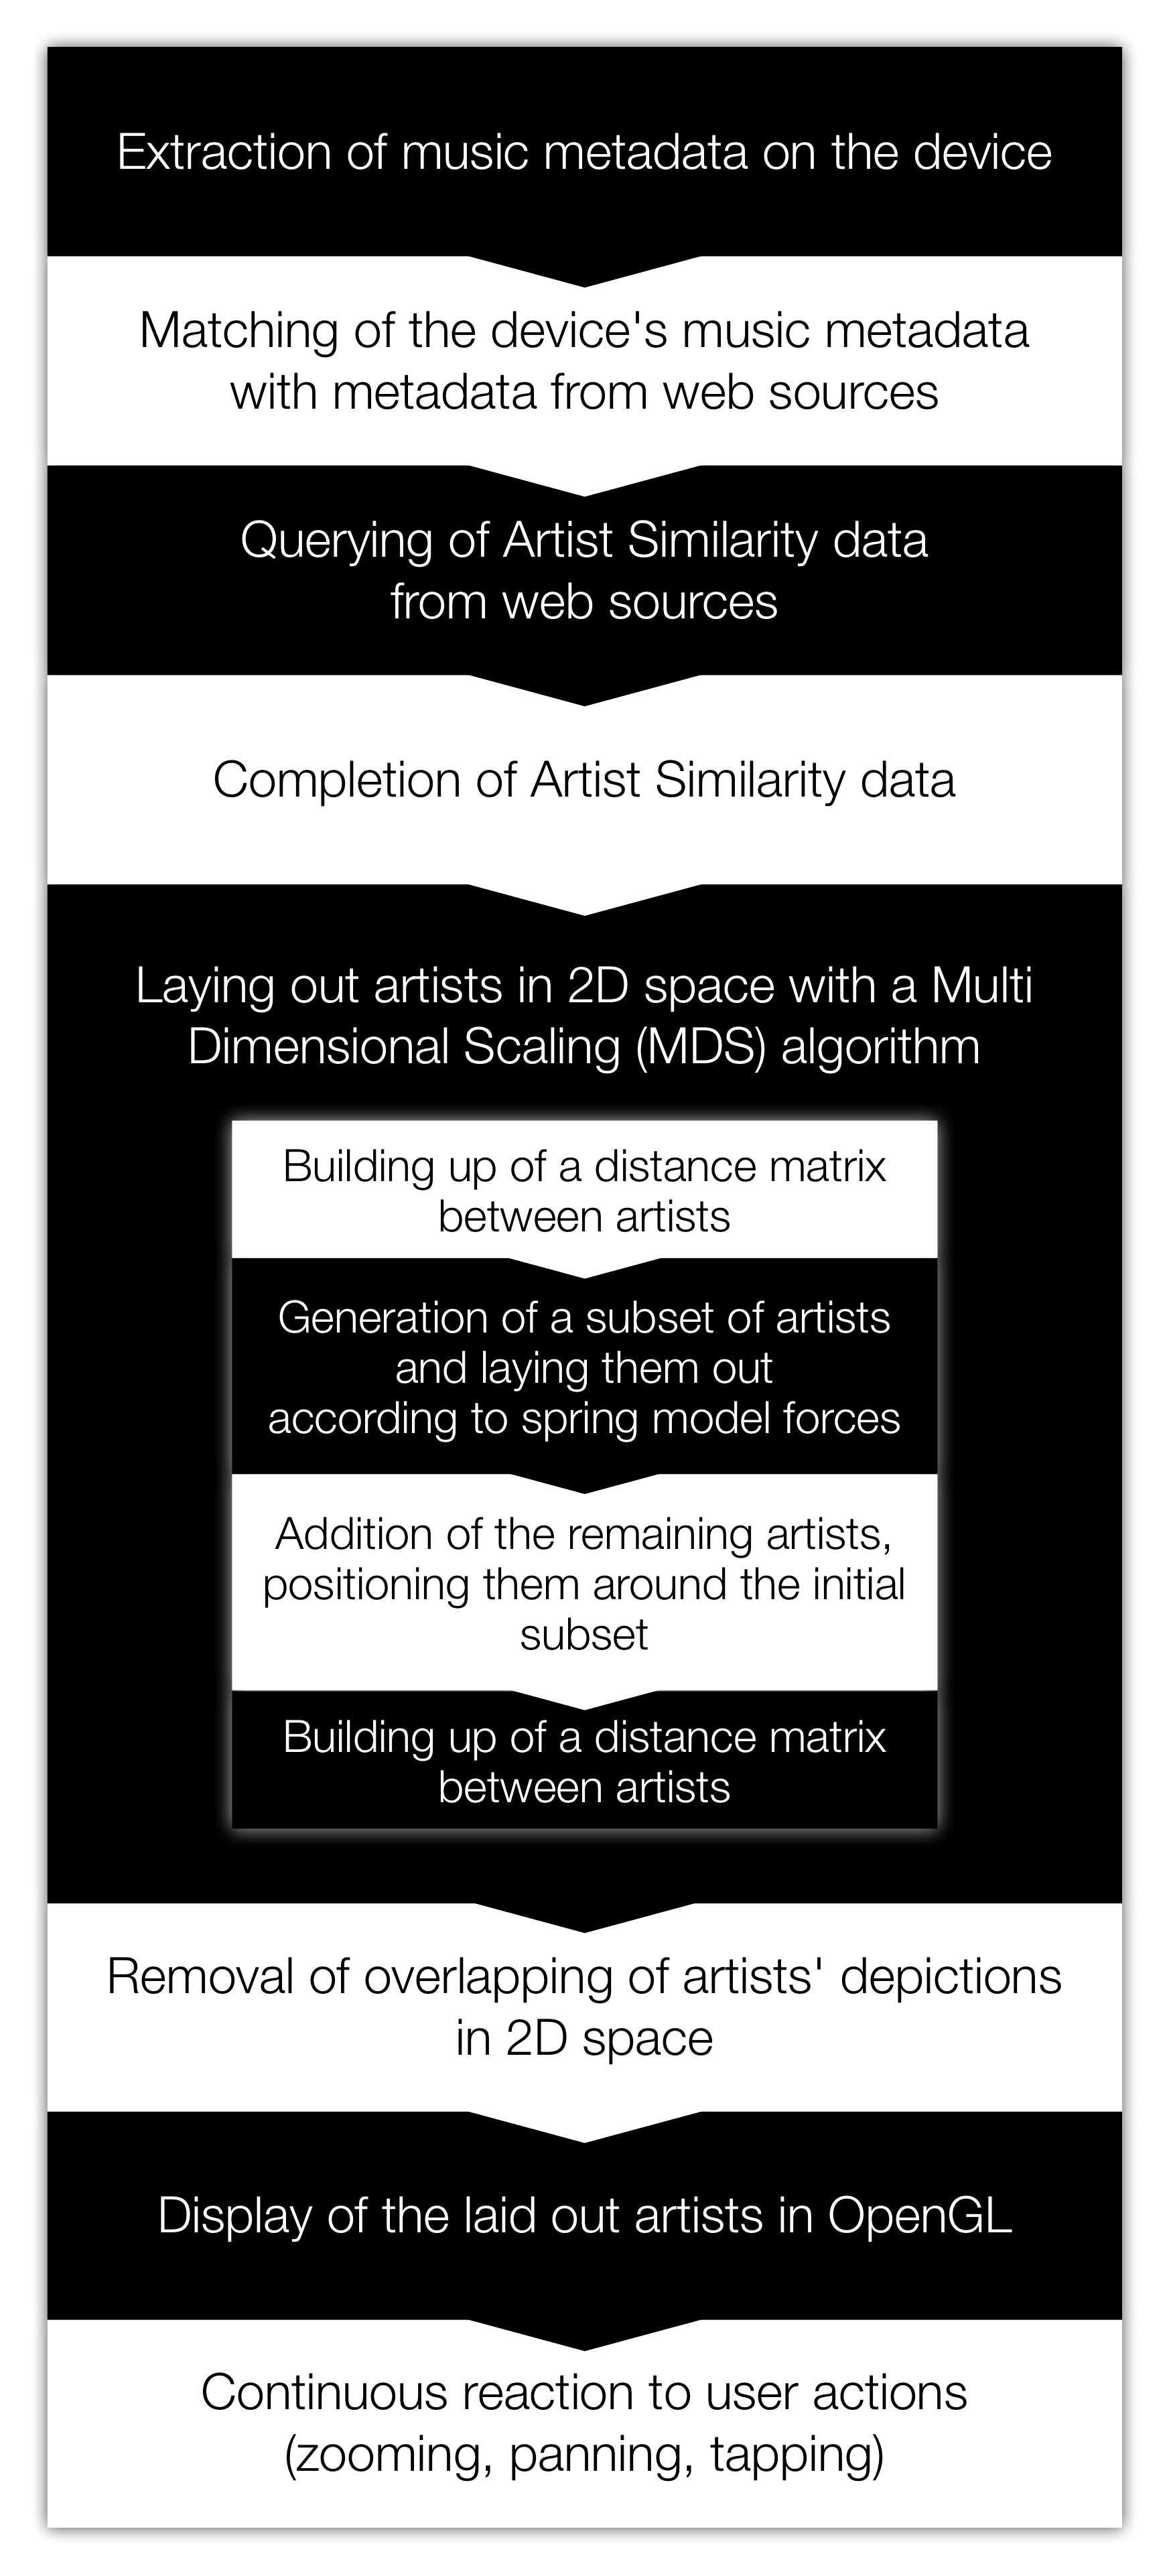
\includegraphics[width=0.45\textwidth]{figures/algorithm_flow_visualization}
  \caption{Algorithms for Library Visualization}
  \label{fig:algorithm_flow_visualization}
\end{figure}

\subsection{Artist Discovery}

Artist discovery is initiated by the user selecting a certain artist ("'subject"'), and requesting discovery mode.

\begin{figure}[H]
  \centering
    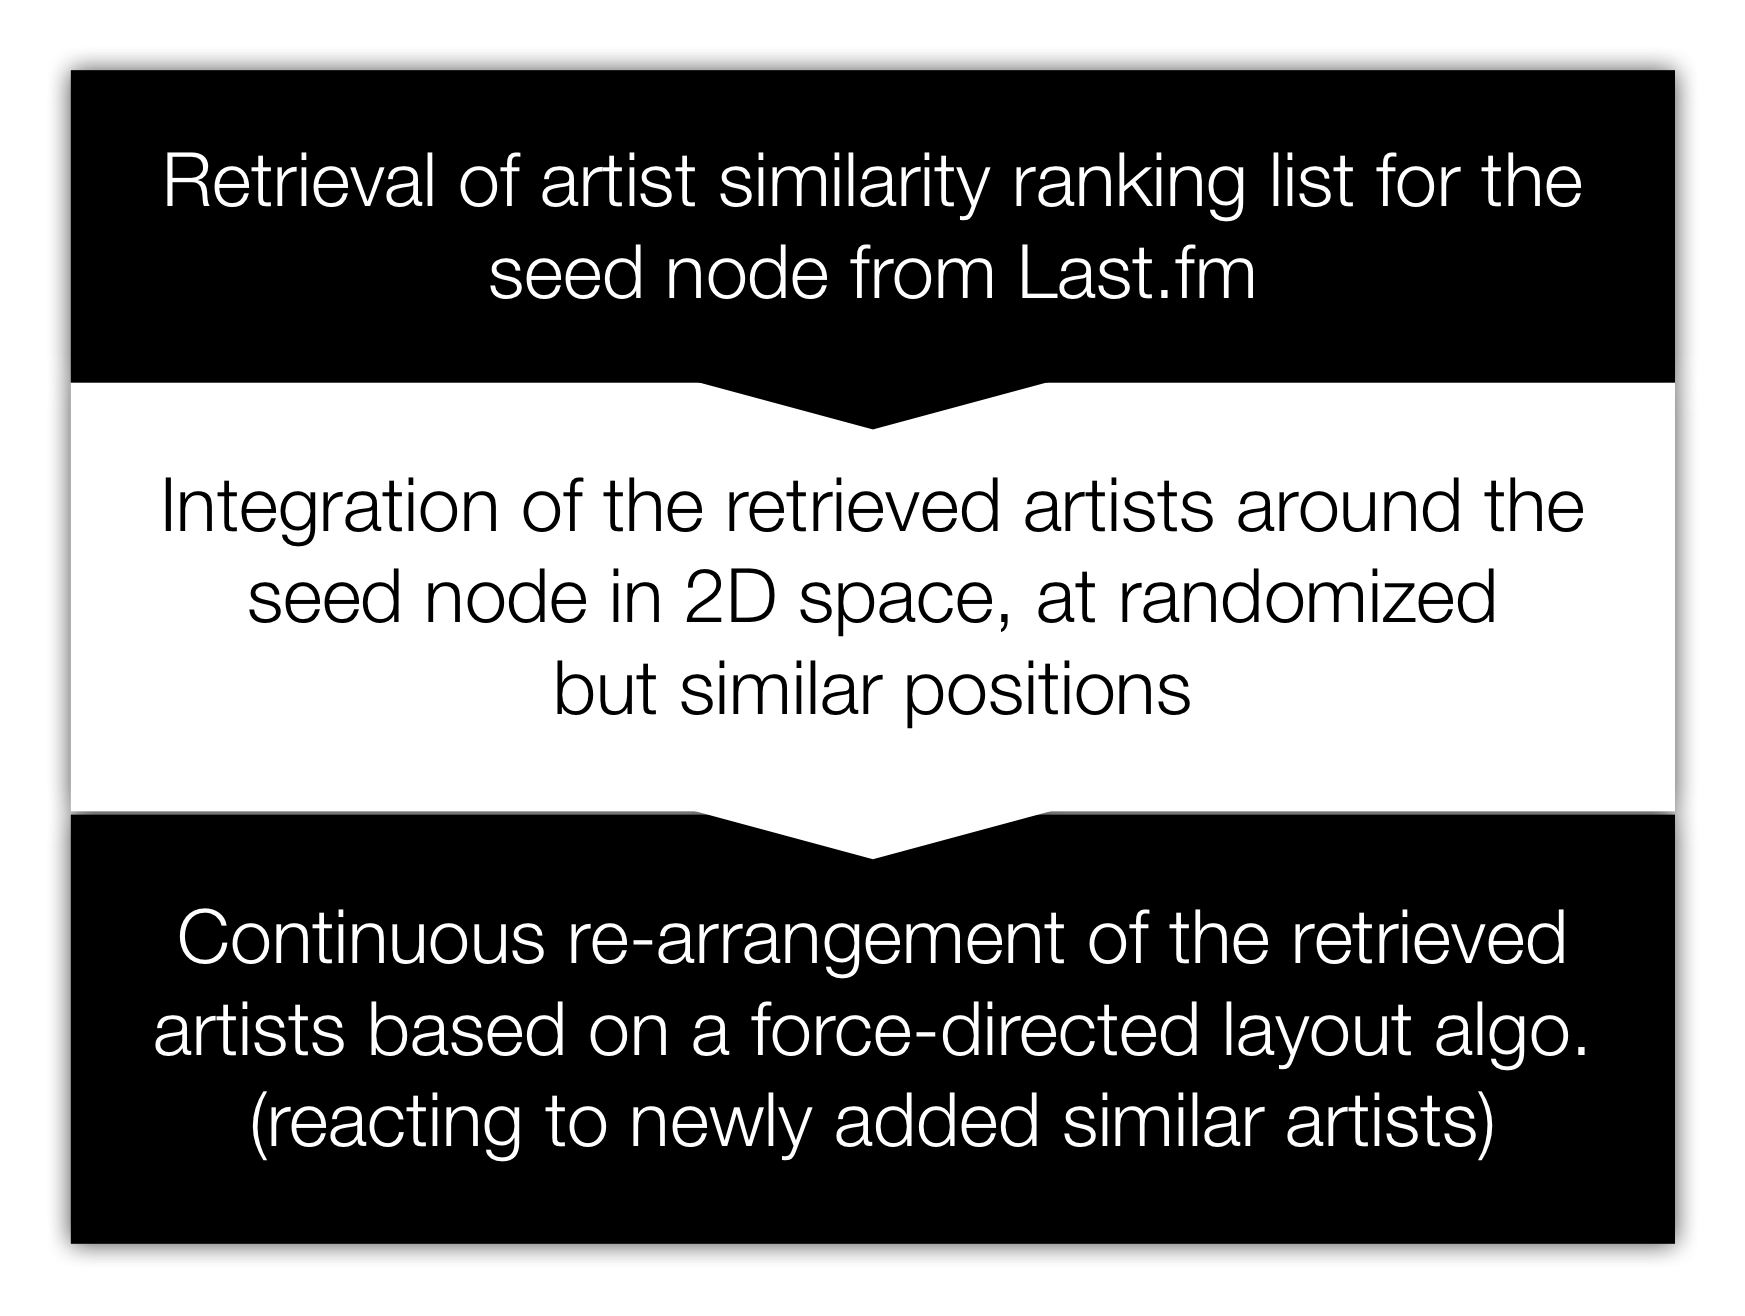
\includegraphics[width=0.45\textwidth]{figures/algorithm_flow_artist_discovery}
  \caption{Algorithms for Artist Discovery}
  \label{fig:algorithm_flow_artist_discovery}
\end{figure}

\section{Summary}

After the definition of the scope of this thesis (verification of artist similarity computational methods and implementation in a prototype), algorithms have been selected for further treatment which have already been outlined in Chapter ~\ref{ch:relatedwork}. For the computation of artist similarity, a multi-dimensional scaling method has been chosen, and the accompanying visualization is highly dependent on the computational part - therefore, a 2D visualization of the MDS output has been selected. 
While the algorithm for the removal of node overlappings in the graph resulting from the previously mentioned computation is a modification of a force-transfer algorithm, the layout computation for artist discovery has been chosen to be force-directed. Finally, an overview of the algorithms and information flow between them has been given, for both artist similarity visualization and artist discovery.